\documentclass[10pt,twocolumn]{article}
\usepackage{graphicx}
\usepackage[spanish]{babel}
\usepackage{amsmath}
\usepackage{amssymb}

\begin{document}
\title{Primer Examen Parcial F\'isica Computacional}
\author{Mauricio Yamil Tame Soria}
\maketitle

\section{P\'endulo invertido(problema 1)}
El p\'endulo es un ejemplo excelente que se usa como modelo para 
estudiar diferentes fen\'omenos f\'isicos. El sistema que propone el 
autor simula un 
p\'endulo r\'igido en dos dimensiones del cual mueven el pivote 
oscil\'andolo peri\'odicamente en forma vertical. Se busca la 
existencia de posiciones invertidas estables para el p\'endulo variando 
los par\'ametros. Cuando se mueve el pivote con una fuerza peri\'odica 
el p\'endulo tiene movimientos oscilatorios y tambi\'en se observan 
movimientos ca\'oticos. El autor estudia el rango de los par\'ametros en 
donde el movimiento invertido se vuelve estable, el an\'alisis se hace 
con ecuaciones linealizadas. La posici\'on invertida estable es un 
fen\'omeno de estabilizaci\'on din\'amica. En los experimentos se 
observa que la posici\'on invertida estable del p\'endulo no es 
completamente vertical si no que tiene un ligero desfase y sugieren que 
se debe a la inclinaci\'on de la fuerza sobre el pivote. Para el 
an\'alisis se utiliza el m\'etodo del potencial efectivo de Kapitza y 
Landau y Lifshitz. Algunas simulaciones num\'ericas muestran la 
relaci\'on entre el \'angulo que se desfasa la posici\'on vertical y el 
\'angulo en el cual se mueve el pivote. Para demostrar la relaci\'on se 
realiza un experimento que consiste en un p\'endulo r\'igido conectado a 
un pivote m\'ovil, donde el movimiento del pivote es movido en un 
movimiento vertical oscilatorio, es decir, de arriba a abajo y as\'i 
peri\'odicamente. A pesar de que se fabricaron instrumentos sim\'etricos 
que brindaban forzamineto vertical a\'un as\'i el estado invertido 
estable no es completamente vertical. El objetivo del autor es discutir 
el estado invertido con m\'as detalle al hacer comparaciones de 
resultados anal\'iticos con soluciones obtenidas num\'ericamente; 
primero consideran el p\'endulo cuando mueven el pivote verticalmente y 
explican c\'omo usar el m\'etodo del potencial efectivo para obtener 
expresiones para la frecuencia en la cual se obtienen posiciones 
invertidas. Despu\'es consideran el sistema con una ligera inclinaci\'on 
en el movimiento del pivote al cual est\'a conectado el p\'endulo y 
obtienen resultados que sugieren que el estado invertido sin 
inclinaci\'on es asint\'otico. \\ \newline
COnstruyen un modelo idealizado del p\'endulo excitado 
param\'etricamente, es decir, se cuantifica la excitaci\'on del pivote. 
El modelo consiste en la masa $m$ unida a una varilla de longitud $l$ 
que est\'a conectada al pivote el cual se mueve sinusoidalmente de 
acuerdo a una ecuaci\'on(funci\'on de posici\'on) $z(\tau)$. Se utiliza 
una 
aproximaci\'on 
lineal de un oscilador amortiguado constantemente(amortiguamineto 
constante $\zeta$), de ah\'i 
obtienen una 
ecuaci\'on

\begin{equation}
	I\frac{d^2\theta}{d\tau^2}+ 2\zeta\frac{d\theta}{d\tau}+\left( g + 
\frac{d^2z}{d\tau^2} \right)\sin\theta=0
\label{osciladoramortiguado}
\end{equation}

que depende del tiempo $\tau$ y del \'angulo respecto a la vertical $\theta$ 
siendo la posici\'on hasta abajo el $\theta=0$. La ecuaci\'on de la 
posici\'on del pivote es un coseno ya que el movimiento del pivote era 
oscilatorio y lo definen as\'i

\begin{equation}
	z(\tau)=-Zcos\Omega\tau
	\label{pospivote}
\end{equation}

haciendo cambio de variables con el tiempo $t=\omega_n\tau$ de tal manera 
que involucran el periodo de oscilaci\'on llegan a una simplificaci\'on

\begin{equation}
	\frac{d^2\theta}{dt^2}+c\frac{d\theta}{dt}+(1+p\cos t\omega)\sin\theta=0 
\label{ecuacion}
\end{equation}

donde 

\begin{equation}
	\omega_n=\sqrt{\frac{g}{l}}, \hspace{0.25cm} \omega=\frac{\Omega}{\omega_n}, \hspace{0.25cm} 
c=\frac{2\zeta}{\omega_nl}, \hspace{0.25cm} p=\frac{Z\Omega^2}{g}
\label{definiciones}
\end{equation}

La ecuacion (\ref{ecuacion} es la que usan en los c\'alculos 
num\'ericos. 
Para el coeficiente de amortiguamiento $\zeta$ utilizan valores que ya conocen. \\ \newline
El valor de $\omega$ que se usa en el articulo para obtener el punto estable $\theta=\pi$ es $\omega=17.5$ 
entonces para estimar el valor de $p$ donde $\theta=\pi$ es estable, se hace la simulaci\'on num\'erica de 
la 
ecuaci\'on (\ref{ecuacion}) resolviendo para $\theta$ con el m\'etodo de Runge-Kutta programado en 
Fortran90(el c\'odigo que est\'a en Dropbox). En el diagrama de bifurcaci\'on que hacen dicen que toman 
una 
muestra cada periodo $T=\frac{2\pi}{\omega}$, editando el c\'odigo RungeKutta.f90 para hacer un diagrama de 
bifurcaci\'on, corriendo con la condici\'on inicial $\theta=3$ por ser un valor cercano a pi, si converge 
$\frac{\theta}{\pi}$ hacia 1 entonceses estable. Observando la gr\'afica supongo que el valor del 
par\'ametro $p$ para el cual $\theta=\pi$ est\'a entre 27.2 y 27.4. 

\begin{figure}[h]
    \centering
	\begin{minipage}{.4\textwidth}
	    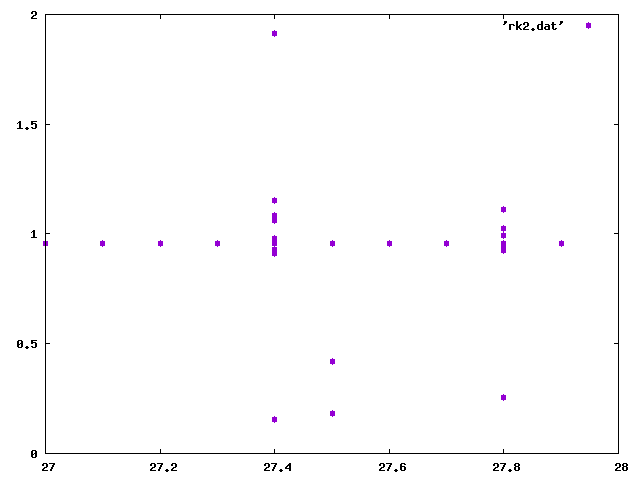
\includegraphics[width=\textwidth]{bif.png}
    	\caption{diagrama de bifurcaci\'on}
	\end{minipage}
\end{figure}


\section{Problema 2}
\subsection{a)}
la ecuaci\'on que se debe resolver es
\begin{equation}
	v'-\frac{c_1}{m}v=-g
	\label{name}
\end{equation}
sabemos que la soluci\'on es $v_h +v_p$ donde $v_h$ es soluci\'on al sistema homog\'eneo y $v_p$ es una 
soluci\'on particular. Para $v_h$ la soluci\'on es $v_h=ke^{-\frac{c_1}{m}t}$ y la soluci\'on particular es 
$v_p=-\frac{m}{c_1}g$ por lo tanto la soluci\'on general es $v=ke^{-\frac{c_1}{m}}-\frac{m}{c_1}g$. Con la 
condici\'on  inicial obtenemos $k$ entonces $v(0)=k-\frac{m}{c_1}g=v_0$ por lo tanto $k=v_0+\frac{m}{c_1}g$ 
de 
esta manera la soluci\'on es 

\begin{equation}
	v=\left(v_0+g\tau\right)e^{-\frac{t}{\tau}}-v_t
\label{sol}
\end{equation}

\subsection{b)}
las unidades de $c_1$ y $c_2$ deben ser $\frac{kg}{s}$ son unidades de masa sobre tiempo.

\subsection{c) y d)}
La ecuaci\'on cuadr\'atica ser\'ia
\begin{equation}
	mv'=-mg-c_2v^2
\label{cuad}
\end{equation}

esta es una ecuaci\'on de ricati, de la cual la soluci\'on es 

\begin{equation}
	v=-\sqrt{\frac{gm}{c_2}}\tan\left(\sqrt{\frac{gc_2}{m}}(k+t)\right)
\label{solcua}
\end{equation} 

$k$ es una constante. En t\'erminos de $\tau$ y $v_t$ la ecuaci\'on queda

\begin{equation}
	v=-v_t\tan\left(\frac{(c_1+t)}{\tau}\right)
\label{solcua}
\end{equation} 
\end{document}
